% Chapter Template

\chapter{Diseño e Implementación} % Main chapter title

\label{Chapter3} % Change X to a consecutive number; for referencing this chapter elsewhere, use \ref{ChapterX}
En el siguiente capítulo se presentará el diseño y la implementación de las tres partes fundamentales del equipo. Se abarcarán aspectos de hardware, firmware, diseño y fabricación mecánica.
%----------------------------------------------------------------------------------------
%	SECTION 1
%----------------------------------------------------------------------------------------

\definecolor{mygreen}{rgb}{0,0.6,0}
\definecolor{mygray}{rgb}{0.5,0.5,0.5}
\definecolor{mymauve}{rgb}{0.58,0,0.82}
%%%%%%%%%%%%%%%%%%%%%%%%%%%%%%%%%%%%%%%%%%%%%%%%%%%%%%%%%%%%%%%%%%%%%%%%%%%%%
% parámetros para configurar el formato del código en los entornos lstlisting
%%%%%%%%%%%%%%%%%%%%%%%%%%%%%%%%%%%%%%%%%%%%%%%%%%%%%%%%%%%%%%%%%%%%%%%%%%%%%
\lstset{ %
  backgroundcolor=\color{white},   % choose the background color; you must add \usepackage{color} or \usepackage{xcolor}
  basicstyle=\footnotesize,        % the size of the fonts that are used for the code
  breakatwhitespace=false,         % sets if automatic breaks should only happen at whitespace
  breaklines=true,                 % sets automatic line breaking
  captionpos=b,                    % sets the caption-position to bottom
  commentstyle=\color{mygreen},    % comment style
  deletekeywords={...},            % if you want to delete keywords from the given language
  %escapeinside={\%*}{*)},          % if you want to add LaTeX within your code
  %extendedchars=true,              % lets you use non-ASCII characters; for 8-bits encodings only, does not work with UTF-8
  %frame=single,	                % adds a frame around the code
  keepspaces=true,                 % keeps spaces in text, useful for keeping indentation of code (possibly needs columns=flexible)
  keywordstyle=\color{blue},       % keyword style
  language=[ANSI]C,                % the language of the code
  %otherkeywords={*,...},           % if you want to add more keywords to the set
  numbers=left,                    % where to put the line-numbers; possible values are (none, left, right)
  numbersep=5pt,                   % how far the line-numbers are from the code
  numberstyle=\tiny\color{mygray}, % the style that is used for the line-numbers
  rulecolor=\color{black},         % if not set, the frame-color may be changed on line-breaks within not-black text (e.g. comments (green here))
  showspaces=false,                % show spaces everywhere adding particular underscores; it overrides 'showstringspaces'
  showstringspaces=false,          % underline spaces within strings only
  showtabs=false,                  % show tabs within strings adding particular underscores
  stepnumber=1,                    % the step between two line-numbers. If it's 1, each line will be numbered
  stringstyle=\color{mymauve},     % string literal style
  tabsize=2,	                   % sets default tabsize to 2 spaces
  title=\lstname,                  % show the filename of files included with \lstinputlisting; also try caption instead of title
  morecomment=[s]{/*}{*/}
}

\section{Hardware}
\subsection{Diseño basado en módulos de hardware libre}

Para la implementación del hardware se utilizó el software libre de diseño de circuitos impresos KICAD \citep{web_kicad}, que en sus últimas versiones presenta mejoras significativas respecto a sus predecesoras.

El diseño de la placa electrónica se baso en el estudio de los siguientes módulos:
\begin{itemize}
\item NodeMCU \citep{web_nodemcu}
\item TMC5130-EVAL \citep{3_web_trinamic_placa}	
\end{itemize}
Se destaca que ambos proyectos adhieren a la filosofía del hardware libre por lo tanto se pudieron descargar y estudiar los diagramas esquemáticos de ambas placas. 

El módulo TMC5130-EVAL como se describió en la sección \ref{sec:Circuitos integrados Trinamic} contiene al CI TMC5130. Del estudio de esta placa de evaluación se extrajeron las configuraciones necesarias para lograr la correcta utilización del driver. Se tuvieron en cuenta las recomendaciones de diseño establecidas por el fabricante como por ejemplo la incorporación de un clock externo de 16 MHz como se observa en la figura \ref{fig:kicad_clock} el cual es necesario en aplicaciones de alta precisión. 

\begin{figure}[h]
	\centering
	\includegraphics[width=.5\textwidth]{./Figures/kicad_clock.png}
	\caption{Clock para el CI TMC5130.}
	\label{fig:kicad_clock}
\end{figure}

Otra etapa importante como se observa en la figura \ref{fig:kicad_tension} es el regulador de tensión que permite alimentar al equipo con tensiones continuas entre 24 V y 46 V.
El equipo se diseño para ser alimentado con una fuente de alimentación externa simplificando así cuestiones regulatorias de certificación que deben cumplir equipos que se alimentan directamente con 220 V de tensión alterna.

\begin{figure}[h]
	\centering
	\includegraphics[width=1\textwidth]{./Figures/kicad_tension.png}
	\caption{Módulo de entrada.}
	\label{fig:kicad_tension}
\end{figure}
 
A continuación observamos en la figura \ref{fig:kicad_trinamic} las conexiones del driver con el motor paso a pasos y el puerto SPI utilizado para la comunicación con el microcontrolador. 
 
\begin{figure}[h]
	\centering
	\includegraphics[width=1\textwidth]{./Figures/kicad_trinamic.png}
	\caption{CI TMC5130.}
	\label{fig:kicad_trinamic}
\end{figure} 
 
El cuanto al módulo NodeMCU es una placa de desarrollo que contiene el SoC ESP32-WROOM, del estudio de su diseño se implementó la etapa del conversor SERIAL-USB como se observa en la figura \ref{fig:kicad_conversor} que permite conectar el módulo directamente a un puerto USB de computadora para descargar el firmware y establecer una comunicación a través del periférico UART. Esto nos evita tener que contar con un programador externo para comunicarnos con el equipo.
\begin{figure}[h]
	\centering
	\includegraphics[width=1\textwidth]{./Figures/kicad_conversor.png}
	\caption{Conversor UART-USB.}
	\label{fig:kicad_conversor}
\end{figure}

%\begin{figure}[h]
%	\centering
%	\includegraphics[width=.6\textwidth]{./Figures/kicad_esp.png}
%	\caption{Módulo ESP32.}
%	\label{fig:kicad_esp}
%\end{figure}
  
Finalmente podemos observar en la figura \ref{fig:dip_3d_model} el diseño 3D generado por el software KICAD cuyo diseño esta disponible en los repositorios de la empresa TECSCI \citep{web_hardware_tecsci}. La placa electrónica de este equipo dip coater cuenta con licencia CERN OHL v.1.2 \citep{web_cern_licence}.


\begin{figure}[h]
	\centering
	\includegraphics[width=.5\textwidth]{./Figures/dip_3d_model.pdf}
	\caption{Modelo 3D Kicad.}
	\label{fig:dip_3d_model}
\end{figure}
         



  
%-----------------------------------
%	SUBSECTION 1
%-----------------------------------
\subsection{Fabricación}
%-----------------------------------
%	SUBSECTION 2
%-----------------------------------
La placa electrónica se fabricó con el proveedor local de circuitos impresos Ernesto Mayer S.A. \citep{web_mayer}. A continuación se presenta la información de diseño de la placa y de describen algunas  restricciones de diseños impuestas por el fabricante:

\begin{itemize}

\item Grilla de posicionamiento principal: 0.25mm
\item Grilla de ruteo principal: 0.25mm
\item Agujeros de montaje: 3.2mm
\item Pistas principales: 0.5mm
\item Pistas inferiores: 0.25mm (límite particular 8mils(0.20mm))
\item Pistas superiores: 0.8mm
\item Vías: 0.8mm/0.4mm (límite particular 8mils(0.20mm))
\item Margen general: 0.22 mm
\item Margen particular: 0.2 mm (límite particual 8 mils(0.20mm))
\item Fabricación: espesor 1.6mm FR4  
\item Restricciones generales del fabricante: estándar 10 mils

\end{itemize}

Luego de fabricar el PCB, se continuó con el montaje de componentes electrónicos superficiales que estuvo a cargo de la empresa Asembli S.A. \citep{web_asembli}. Se fabricó un primer lote de cinco placas.


\begin{figure}[htbp]
	\centering
	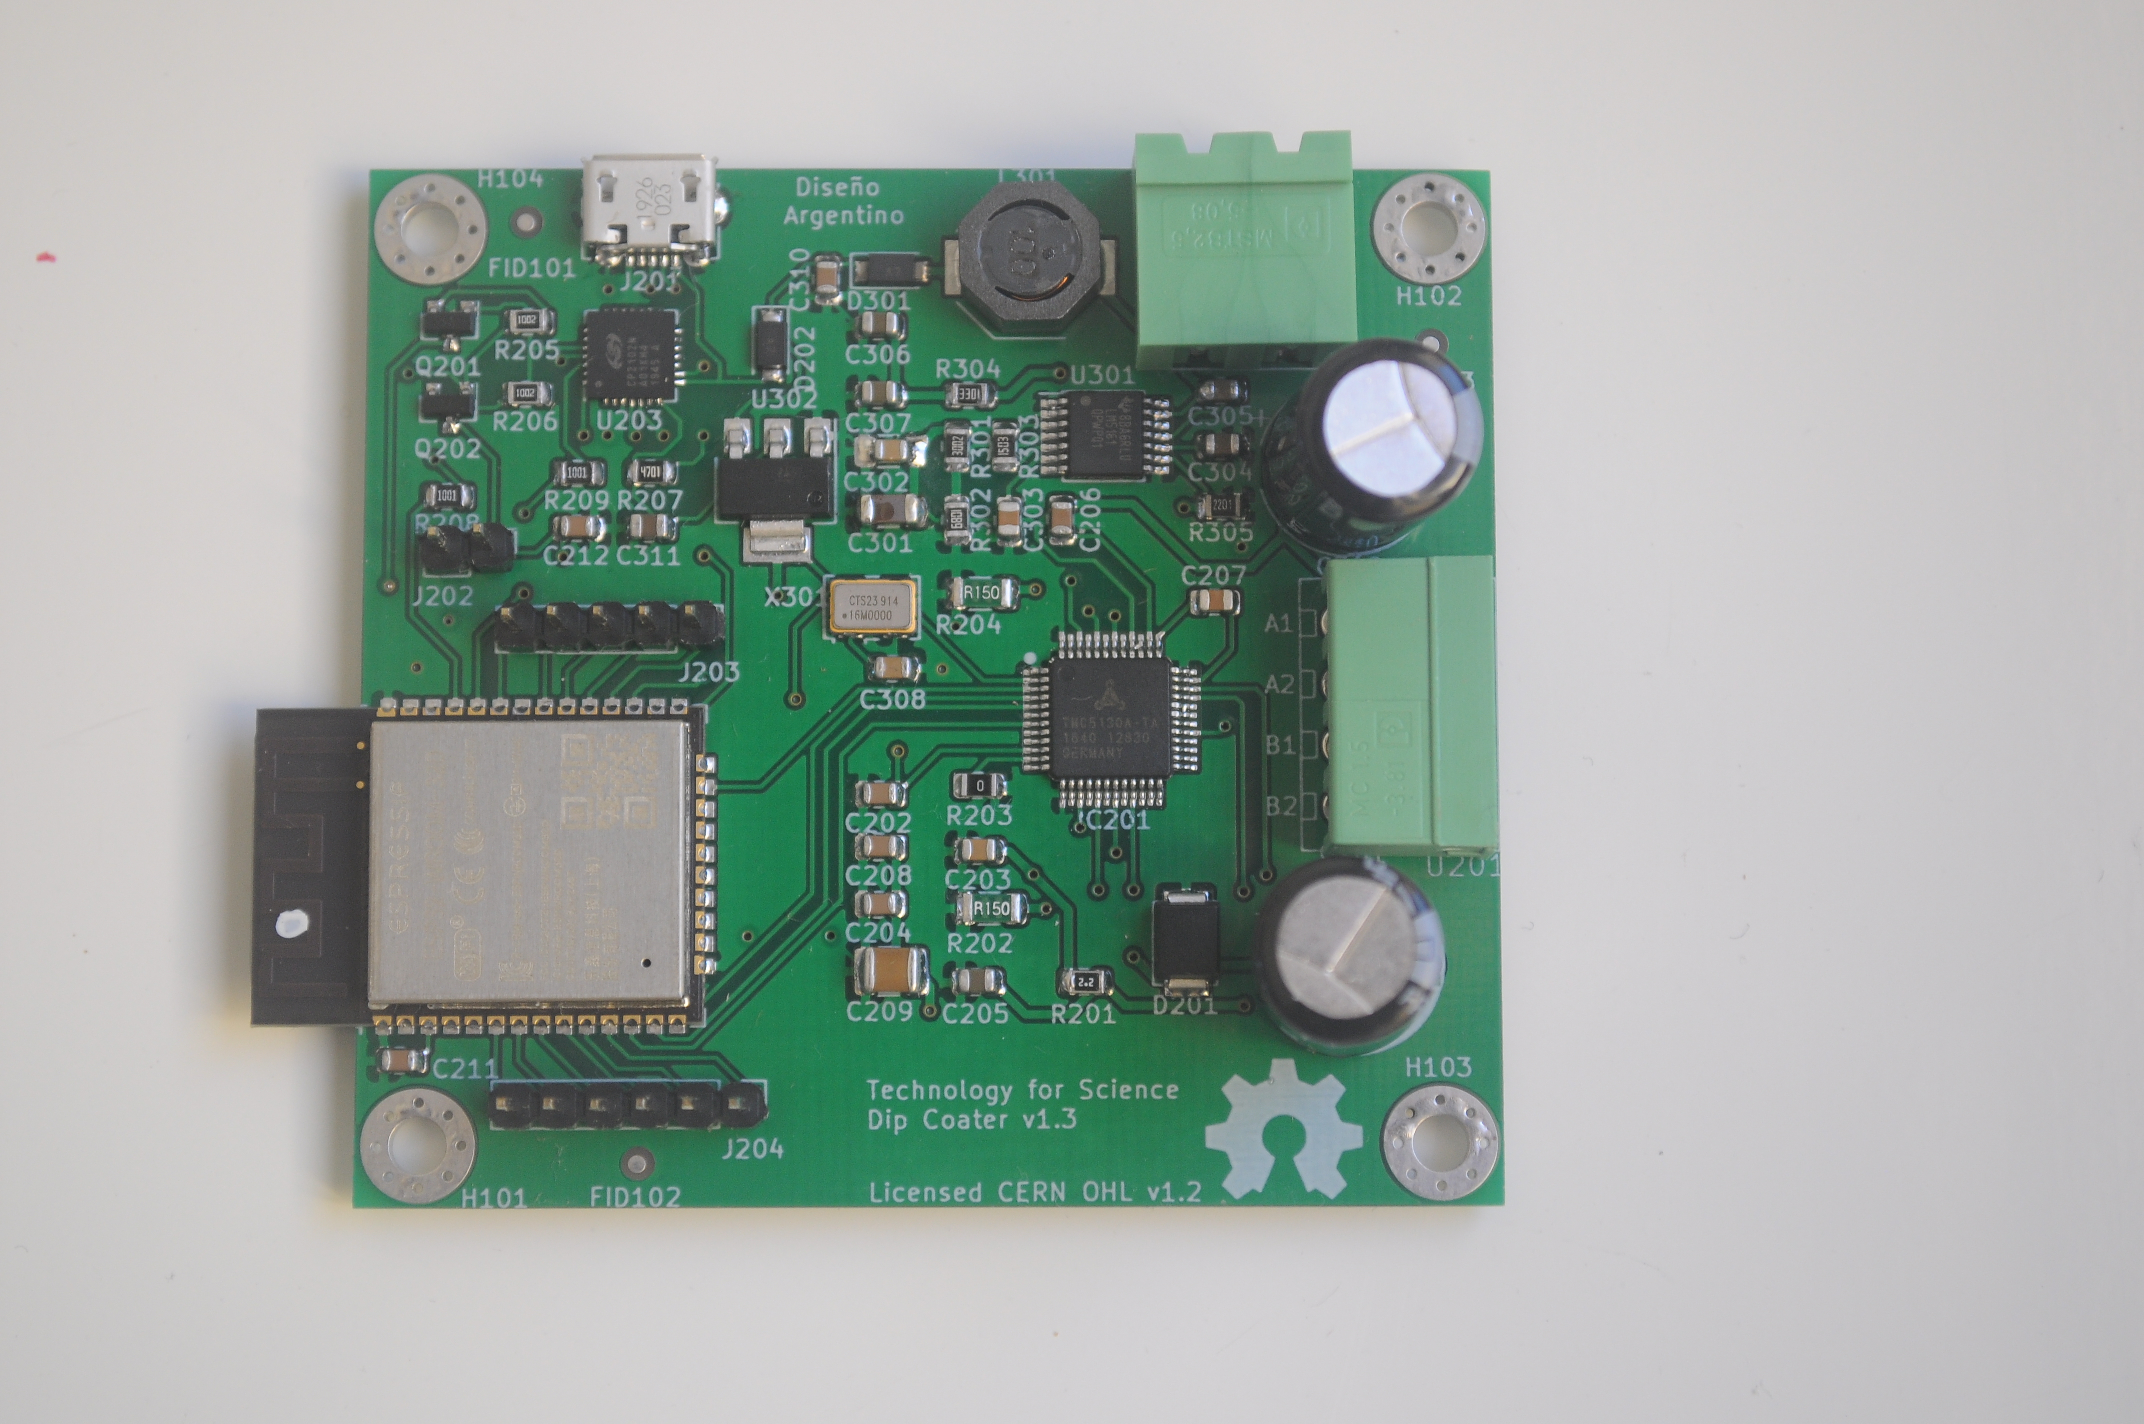
\includegraphics[width=1\textwidth]{./Figures/dip_real_model.png}
	\caption{Placa fabricada MAYER SRL.}
	\label{fig:dip_real_model}
\end{figure}

%----------------------------------------------------------------------------------------
%	SECTION 2
%----------------------------------------------------------------------------------------

\section{Firmware}
\subsection{Capas de abstracción}

Para la implementación del firmware se trabajo con el \textit{framework} ESP-IDF FreeRTOS \citep{web_esp_idf} provisto por el fabricante del microcontrolador. FreeRTOS es un sistema operativo de tiempo real que permite la programación de software \textit{multi-threaded}. En la sección \ref{sec:Módulos principales} se detallarán los módulos del framework utilizados. 

Se desarrollo un firmware modular que atomiza el funcionamiento en diferentes bloques de software, lo cual permite incorporar código de manera incremental y ordenada. Se observa en la figura \ref{fig:capas} las capas de abstracción de software implementadas.

La idea principal es no permitir llamados a funciones entre capas que no son continuas.La capa superior de aplicaciones solo puede hacer llamados a funciones de la capa dos o capa \textit{API(Application Programming Interfaces)} y la capa dos solo puede hacer llamado a funciones de la capa inferior o capa \textit{Board}.


\begin{figure}[h]
	\centering
	\includegraphics[width=1\textwidth]{./Figures/capas.jpg}
	\caption{Capas de abstracción de software.}
	\label{fig:capas}
\end{figure}

La capa uno interacciona con los módulos de hardware del microcontrolador, es decir que esta capa es la única que contiene todos los llamados a funciones disponibles en el framework ESP-IDF, como por ejemplo llamados a periféricos  UART , SPI, I2C entre otros. En el caso de que en un futuro se quiera realizar un cambio de microcontrolador, esta sería la única capa que debería reescribirse en mayor medida, permitiendo así reutilizar el software escrito en capas superiores.

La capa dos esta compuesta por bloques de código provistos por los fabricantes de drivers, como por ejemplo API-TMC que es una api provista por el fabricante trinamic y adaptada a este firmware. También la API-BOSH fue provista por el fabricante y adaptada a este firmware. Y también por una API especifica de este firmware con contiene lógica de código como por ejemplo el manejo de programas guardados en memoria interna. 


La capa tres corresponde a la capa de aplicaciones, el firmware cuenta con 3 aplicaciones fundamentales para el funcionamiento del equipo y una aplicación de test utilizada para probar nuevos componentes y realizar test sobre el sistema que se activa y desactiva según la necesidad de uso.
La aplicación app coating contiene toda la lógica de control de movimientos, es la aplicación que controla los movimiento del equipo

Las aplicaciones app consola y app hmi se encargan de la comunicación con el usuario del equipo.

\subsection{Módulos principales}
\subsubsection{Módulo coating}
\subsubsection{Módulo de consola}
\subsubsection{Módulo hmi}
\subsubsection{Módulo de calibración}

La carpeta /components/config contiene tres archivos de configuración importantes, hardware.h contiene todos las macros referidas a los pines de conexión del modelo de microcontrolador utilizado, os config.h contiene las macros de configuración de las tareas de FreeRTOS tal es el caso de tamaños, prioridades, y periodos de tiempo.
Por último machine.h contiene las macros relacionadas con la calibración del equipo. La macro mas importante es MACHINE STEPS PER MILLIMETER y es muy importante que este bien definida, en la sección cuatro(llenar) se demuestra el procedimiento realizado para definir su valor. Esta macro define cuantos micropasos del motor son necesarios para generar un desplazamiento de 1 mm. Con este valor de micropasos por milímetro se pueden calcular los factores de correcion de unidades. Es decir, los registros del driver TMC5130 para posición son expresados en la unidad de micropados, para la velocidad utiliza micropasos sobre segundos y para la aceleracion micropasos sobre segundos al cuadrado.

Como se analiza en la hoja de datos del driver \citep{3_web_trinamic_producto}  en el capitulo () para lograr es importante conteplar en el calculo la velocidad de clock externo incorporado.

Como se mencionon en la seccion () el equipo de configuro con 51200 micropasos.  
 
 

\begin{lstlisting}[label=cod:vControl,caption=Pseudocódigo del lazo principal de control.]  % Start your code-block
/*Buscar este numero con calibración mecánica del sistema*/

#define MACHINE_STEPS_PER_MILLIMETER	(12916)		
#define MACHINE_EXT_CLOCK				(16000000)	//16MHz


/*FACTOR*/
/*((MACHINE_EXTERNAL_CLOCK/2)*(1/8388608))*/	
#define MACHINE_USTEPS_VELOCITY_FACTOR	  (0.9536743164)
/*((MACHINE_EXT_CLOCK*MACHINE_EXT_CLOCK)/(512*256)/ (16777216) )*/
#define MACHINE_USTEPS_ACELERATION_FACTOR (116.4153218)


/*UPPER AND LOWER MECHANICAL LIMIT*/

#define MACHINE_CONTROL_MECANICAL_UPPER_LIMIT 	(MACHINE_STEPS_PER_MILLIMETER * 10 ) // 10mm
#define MACHINE_CONTROL_MECANICAL_LOWER_LIMIT	(MACHINE_STEPS_PER_MILLIMETER * 290) // 290mm

\end{lstlisting}


\label{sec:Módulos principales}



%----------------------------------------------------------------------------------------
%	SECTION 3
%----------------------------------------------------------------------------------------

\section{Estructura mecánica}
\subsection{Fabricación de piezas personalizadas a través de mecanizado CNC}

Como se mencionó en la sección \ref{sec:estructura_mecanica} se utilizó para el diseño mecánico del equipo el software BOBCAD. El módulo CAD del software nos permite realizar un modelo 2D y 3D de pieza necesarios para la fabricación. El prototipo de dip coater cuenta actualmente con dos piezas mecanizadas. Podemos observar en la figura \ref{fig:carro} la pieza que se acopla al carro de la guiá lineal presentada en la sección \ref{sec:estructura_mecanica}.

\begin{figure}[ht]
	\centering
	\includegraphics[width=.5\textwidth]{./Figures/3d_carro.png}
	\caption{Pieza personalizada soporte de carro.}
	\label{fig:carro}
\end{figure}

Y en la figura \ref{fig:estructura_superior} el soporte superior que sostiene el motor paso a pasos y el  tornillo que esta acoplado al eje del motor.

\begin{figure}[ht]
	\centering
	\includegraphics[width=.5\textwidth]{./Figures/3d_top.png}
	\caption{Piezas personalizada soporte de estructura superior.}
	\label{fig:estructura_superior}
\end{figure}

Con el modelo 3D diseñado se fabricó una primera versión a través de impresión 3D en plástico, luego que las piezas fueron probadas, testeadas y aprobadas en el prototipo se paso a la fabricación en aluminio.

La estrategia utilizada en el mecanizado es por el método de arranque de viruta, es decir que se parte de un bloque de aluminio con material suficiente y las herramientas de corte van penetrando y desventando el bloque hasta lograr la pieza. Esta estrategia se programa en la parte CAM del software, se puede observar en la figura \ref{fig:estrategia} un listado de todas las operaciones que se van definiendo en la programación.

\begin{figure}[ht]
	\centering
	\includegraphics[width=.6\textwidth]{./Figures/3d_estrategia.png}
	\caption{Estrategias de mecanizado en software Bodcad.}
	\label{fig:estrategia}
\end{figure}

Existen diferentes funciones para diferentes tipos de operaciones tal es el caso de refrentado, vaciado, fresado de chaflán, taladros y muchas más. Cada una de estas funciones en general son realizadas por herramientas específicas que son definidas en la configuración del software.
Estas piezas fueron fabricadas en dos etapas, primero se mecanizo la parte superior de la pieza y luego de una rotación de  180° y otro programa se mecanizo la parte inferior.



\subsection{Modelos 3D y real}

A continuación en la figura \ref{fig:mecanica_3d_model} se presenta el primer modelo 3D diseñado de equipo dip coater.
\begin{figure}[h]
	\centering
	\includegraphics[width=1\textwidth]{./Figures/3d.jpg}
	\caption{Modelo 3D.}
	\label{fig:mecanica_3d_model}
\end{figure}

Se detallan a continuación los siguientes componentes fundamentales del equipo:

\begin{itemize}
\item Guiás lineales IGUS 
\item Mecanizado soporte superior y mecanizado carro
\item Placa electrónica
\item Pantalla táctil 4.3 inch
\end{itemize}

Luego de sucesivas iteraciones con pruebas de piezas impresas en material plástico se logró fabricar un primer prototipo completamente en metal que se presenta a continuación en la figura \ref{fig:mecanica_real_model}.

\begin{figure}[h]
	\centering
	\includegraphics[width=0.75\textwidth]{./Figures/real.png}
	\caption{Primer prototipo dip coater TECSCI.}
	\label{fig:mecanica_real_model}
\end{figure}

